\section{Secondary figures and results}
\label{sec:app_secondary}

The figures and analyses that support Section~\ref{sec:results} but that its claims do not need on the page.

\subsection{Carrying}

\begin{table}[htbp]
\centering
\footnotesize
\setlength{\tabcolsep}{2.6pt}
\caption[The carry in the twin on 1\,m cables]{The carry arm with 1\,m cables, as Table~\ref{tab:T7t}: two runs per
cell, the range over the two runs.}
\label{tab:T7t1m}
\begin{tabular}{llccccccc}
\toprule
 & & \multicolumn{2}{c}{Scored} & \multicolumn{5}{c}{Reported} \\
\cmidrule(lr){3-4}\cmidrule(lr){5-9}
 & Speed & Ring RMSE & Peak tilt & Path RMSE & Path tilt & Cut & Across rms & Lag \\
Path & (m/s) & (mm) & ($^\circ$) & (mm) & ($^\circ$) & (mm) & (mm) & (ms) \\
\midrule
Circle & 0.125 & 10.3--11.1 & 1.8 & 4.8--5.8 & 0.9--1.0 & 2.3--3.3 & 2.9--3.9 & 63--82 \\
Circle & 0.2 & 12.1--12.4 & 1.8--2.0 & 9.3--9.4 & 1.4--1.7 & 6.8--7.7 & 9.4--9.6 & 72--77 \\
Figure-eight & 0.2 & 14.6--16.0 & 1.7--2.5 & 14.3--15.7 & 1.7--2.3 & 20.4--20.6 & 13.1--14.7 & 36--56 \\
Line & 0.2 & 11.0--12.0 & 1.9--3.0 & 9.6--11.2 & 1.6--3.0 & -- & 1.2 & -- \\
Orbit & 0.2 & 11.9--13.2 & 2.2--2.8 & 11.5--12.6 & 1.8 & 8.2--9.5 & 8.4--9.8 & 48--60 \\
\bottomrule
\end{tabular}
\end{table}

\begin{figure}[h]
\centering
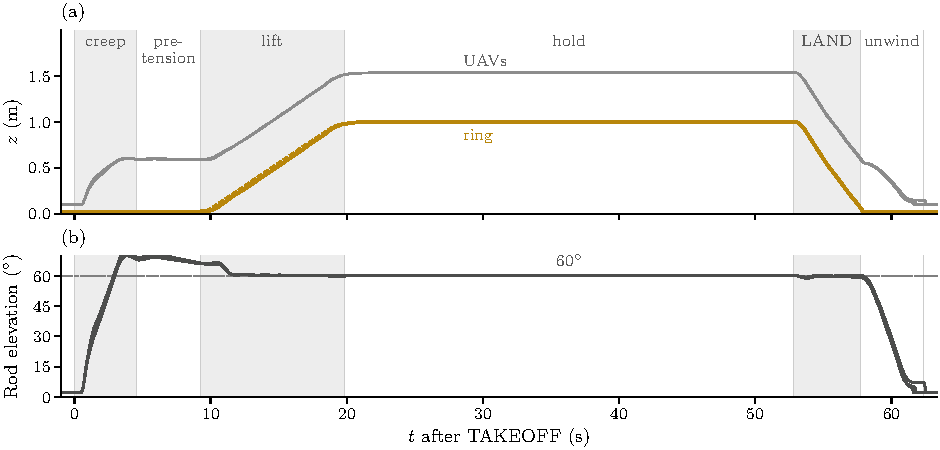
\includegraphics[width=\textwidth]{Images/flight.pdf}
\caption[One flight from the floor]{One flight from the floor in the rig twin: three carriers, hover at 1.0\,m, the
default controller (their traces overlap). (a) Heights of the ring (gold; dashed: its planned height) and of the
UAVs (grey); shaded: the creep, the lift and LAND. (b) Elevation of each rod above the horizontal; dotted: the
planned 60$^\circ$. In the creep the UAVs climb and swing their rods up from the floor, past the planned elevation,
without lifting the ring; in the pretension they hold their height while the rod feedforward eases in; the ring
then leaves the floor and follows its lift ramp to 1.0\,m while the rods settle on 60$^\circ$. On LAND the ring and
the UAVs descend together until the ring is on the floor; the UAVs then unwind along their rods.}
\label{fig:flight}
\end{figure}

\begin{figure}[htbp]
\centering
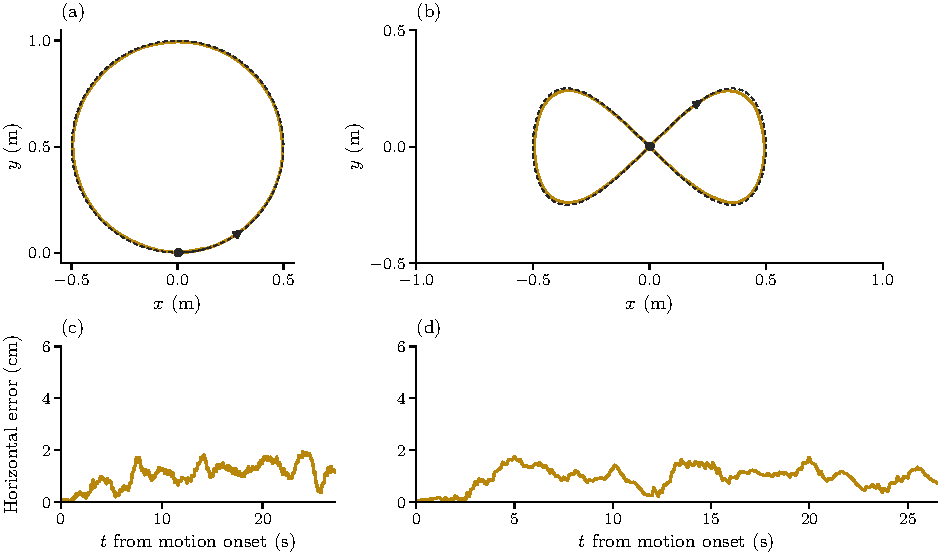
\includegraphics[width=\textwidth]{Images/trajectories.pdf}
\caption[The ring's path in the twin]{The ring's path in the rig twin at the rig's speed: three carriers, 0.125\,m/s
peak path speed, one run of each from the carry claim. (a) The orbit, one lap of radius 0.5\,m; (b) the figure-eight,
$a = 0.5$\,m. Gold: the ring's centre; dashed: the path; dot and arrow: start and direction. (c, d) The ring's
horizontal distance from the planner's reference, sampled at its 10\,Hz updates, from the onset of motion; this
time-indexed error includes the lag, which Table~\ref{tab:T7t} reports apart.}
\label{fig:traj}
\end{figure}

\begin{figure}[htbp]
\centering
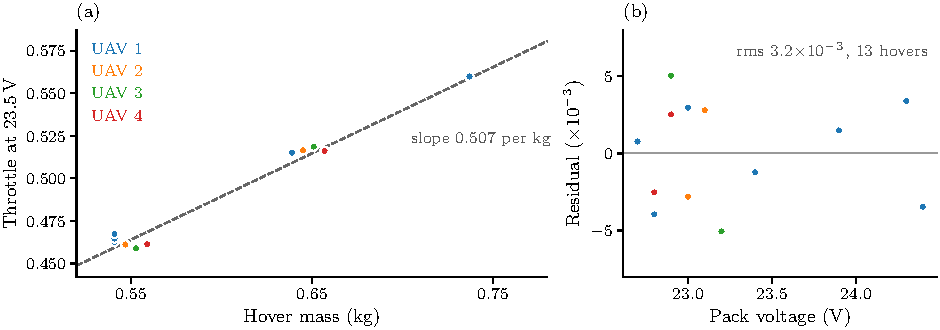
\includegraphics[width=\textwidth]{Images/thrust_map.pdf}
\caption[The rig's thrust map]{The rig's thrust map from 13 free hovers on 30 September, each UAV carrying 0, 98 or
196\,g. (a) Hover throttle corrected to 23.5\,V and to the mean offset, against the hover mass; one colour per UAV
(markers offset sideways by up to 9\,g so that hovers at the same mass can be seen); dashed: the fit
\eqref{eq:thrust_fit} with per-UAV offsets $a_i$ of 0.181--0.187. (b) The residuals of the fit against the pack
voltage: rms $3.2\times10^{-3}$, at most $5\times10^{-3}$ (about 1\,\% of hover throttle), with no trend left in
voltage.}
\label{fig:thrust_map}
\end{figure}

\begin{figure}[htbp]
\centering
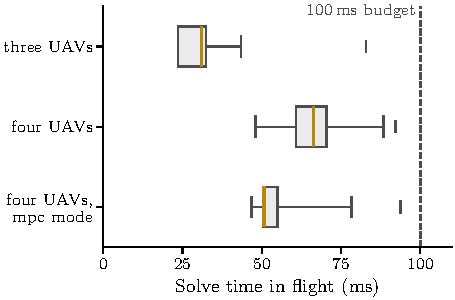
\includegraphics{Images/solve_time.pdf}
\caption[Planner solve time on the rig]{The planner's optimisation time in flight on the rig, 7--8 October:
three UAVs (after a detach, 15\,883 ticks), four UAVs (detach mode, 4\,762 ticks; carry mode, 22\,385 ticks). Box:
quartiles and median (gold); whiskers: 1st and 99th percentile; bar: the slowest tick. Medians 31, 66 and 51\,ms;
99th percentiles 44, 88 and 78\,ms; no tick reached the 100\,ms tick (dashed).}
\label{fig:solve_time}
\end{figure}

\begin{figure}[htbp]
\centering
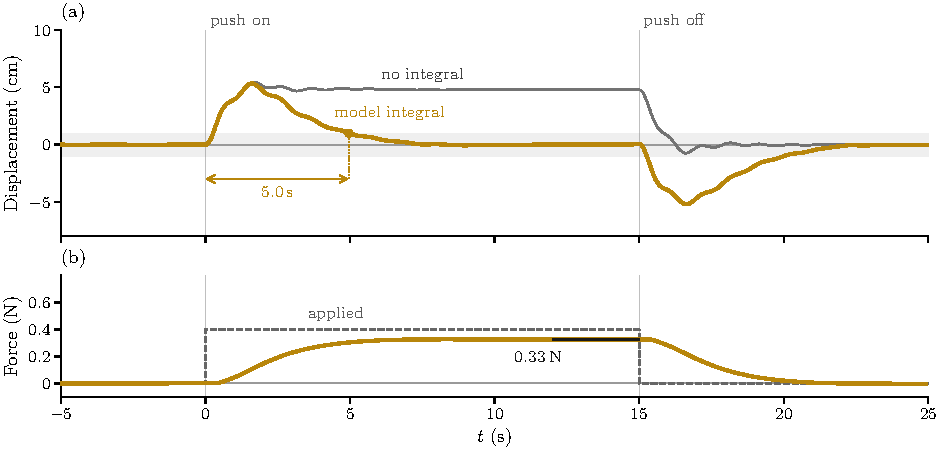
\includegraphics[width=\textwidth]{Images/disturbance.pdf}
\caption[Rejection of a horizontal force on the ring]{Rejection of a constant horizontal force on the ring in the
rig twin: three carriers, hover at 1.0\,m, the measured rod pull; a 0.4\,N push acts from 0 to 15\,s; one run of
each case (Table~\ref{tab:disturbance} gives both runs and the vertical push). (a) Ring displacement along the push,
relative to its mean over the 5\,s before: no integral (grey) and the integral in the planner's model (gold). Band:
$\pm 1$\,cm. Arrow: the time for the model integral to bring the ring back within 1\,cm for good. (b) Change of the
model integral's force $\mathbf{d}$ along the push from its value before the push (gold), against the applied force
(dashed). Black bar: its mean over the last 3\,s of the push.}
\label{fig:disturbance}
\end{figure}

\subsection{Releases on the rig}

\begin{table}[htbp]
  \centering
  \footnotesize
  \caption[The rig release record: conditions]{The hardware release record, conditions (T8a): one row per release
  event, the uncommanded ones included. Layout: the survivors' plates, then the leaver's, and the largest gap left.
  L10 and L11 are the uncommanded releases of the attach flights of 14 and 15 October, with three carriers and the
  fourth UAV not yet attached; they are not yet scored on the frozen metric. [L8 and L9: the next rig day.]}
  \label{tab:T8a}
  \begin{tabularx}{\textwidth}{lYccYYY}
    \toprule
    Event & Release & Pull source & Rod plan & Integral & Layout, largest gap & Freed-UAV policy \\
    \midrule
    L1 & announced & planned & 45$^\circ$ & reference & 3/7/11 + 9, 120$^\circ$ & hovers in place; lands with the fleet \\ % r0012 (7 Oct): no step-out
    L2 & announced, then two uncommanded & planned & 45$^\circ$ & reference & 3/6/11 + 9, 150$^\circ$ & steps out 0.5\,m \\ % r0013 (7 Oct): the rods at 11 and 6 let go 0.17 and 0.39 s after the release; capsize
    L3a & uncommanded, circle & measured & 45$^\circ$ & model & 0/6/9 + 3, 180$^\circ$ & none (carry planner); operator LAND \\ % r200006 slip 1 (7 Oct), four UAVs on the even ring, the rod at plate 3 let go 3.9 s into the orbit
    L3b & uncommanded, in the landing & measured & 45$^\circ$ & model & 0/9 + 6, 270$^\circ$ & none \\ % r200006 slip 2, 2.8 s after slip 1; capsize
    L4 & announced & measured & 60$^\circ$ & reference & 3/7/11 + 9, 120$^\circ$ & steps out 0.5\,m; lands with the fleet \\ % r302_3 (8 Oct), detach_drop.yaml, drop_on_loss armed
    L5 & unannounced & measured & 60$^\circ$ & reference & 3/7/11 + 9, 120$^\circ$ & steps out 0.5\,m; lands with the fleet \\ % r303_4 (8 Oct), drop_and_land.yaml, detect 0.06 m
    L6 & unannounced & measured & 60$^\circ$ & reference & 3/6/11 + 9, 150$^\circ$ & steps out 0.5\,m; lands with the fleet \\ % r304_3 (8 Oct)
    L7 & unannounced, circle & measured & 60$^\circ$ & reference & 3/7/11 + 9, 120$^\circ$ & clears the orbit, lands alone \\ % r305 (8 Oct), departed_land
    L8 & unannounced & measured & 60$^\circ$ & model & 3/7/11 + 9, 120$^\circ$ & lands, disarmed alone \\
    L9 & unannounced, circle & measured & 60$^\circ$ & model & 3/7/11 + 9, 120$^\circ$ & lands, disarmed alone \\
    L10 & uncommanded, in the lift & measured & 60$^\circ$ & model & three carriers, one lost & none: the drop rule was then off in this mode \\ % RIG-1014-t5_2
    L11 & uncommanded, in hover & measured & 60$^\circ$ & model & 3/11 + 7, two left & the drop rule: every carrier lands \\ % RIG-1015-a2_2: QUAD2 let go of plate 7
    \bottomrule
  \end{tabularx}
\end{table}

\begin{figure}[htbp]
\centering
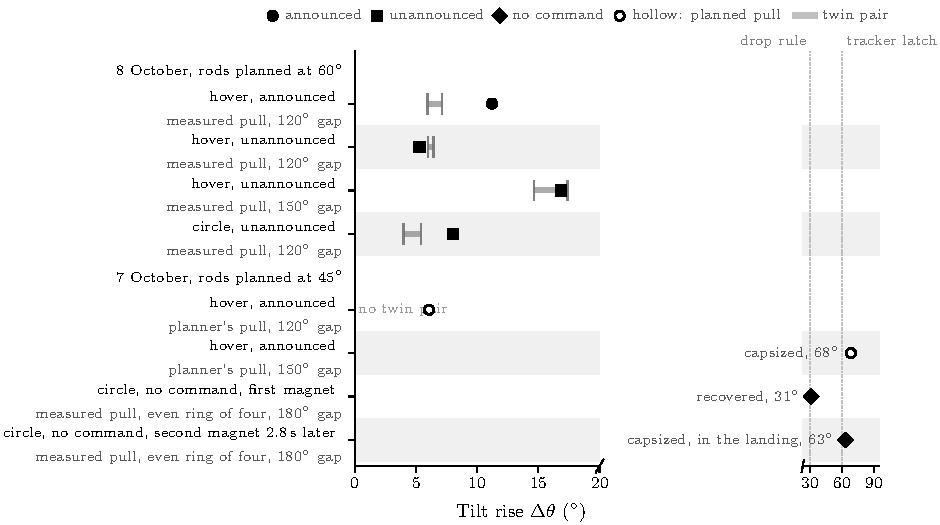
\includegraphics[width=\textwidth]{Images/releases.pdf}
\caption[Every release on the rig]{Every release on the rig to 8 October, one row per event, grouped by the day and
the rod plan: the ring's tilt rise $\Delta\theta$ (the departure of its tilt vector from its mean over the 5\,s
before the event, over the event to LAND or to the fleet's latch) as a marker, filled for the measured rod pull and
hollow for the planner's pull, shaped by how the release came (announced, unannounced, or a magnet letting go with no
command); the grey bar with end ticks is the range of the twin pair flown on the same configuration, cut at the rig
flight's hold, and rows without one say so. The two capsizes and the one recovery sit on the broken axis against the
30$^\circ$ drop rule, which these flights predate, and the trackers' 60$^\circ$ latch. The 7 October circle flew the
even ring of four, whose three survivors leave a 180$^\circ$ gap; it lost two magnets 2.8\,s apart, recovered from the
first, and capsized on the second during the landing, so that row's pre-window holds the first recovery.}
\label{fig:F10}
\end{figure}

\begin{figure}[htbp]
\centering
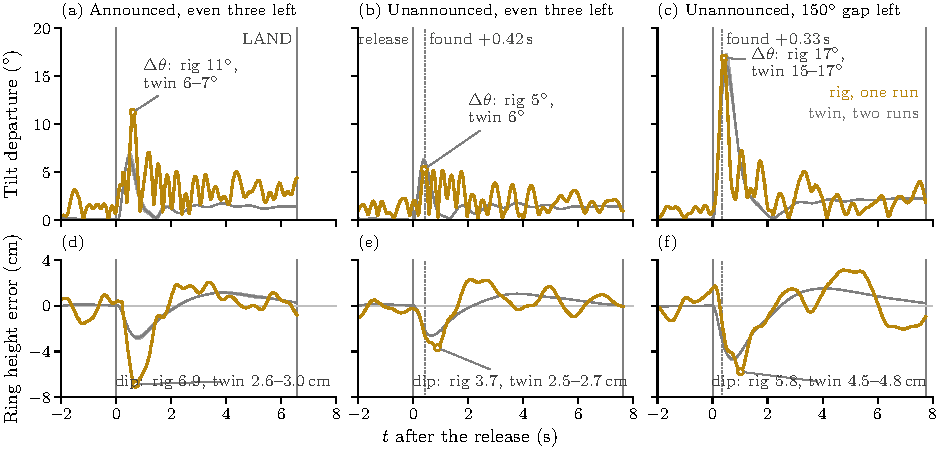
\includegraphics[width=\textwidth]{Images/rig_detach.pdf}
\caption[Releases on the rig against the twin]{Releasing one UAV of four on the rig, 8 October (gold, one run each)
against the rig twin (grey band and line: two runs, nearly identical), aligned on the release (dotted). Announced: the
planner releases the magnet and drops the UAV from its optimisation at once. Unannounced: the magnet is switched off
without telling the planner, which finds the release from the stretched rod (second dotted line, 0.33--0.42\,s after
the release on the rig). (a--c) The ring's tilt departure: the length of its tilt vector's difference from that
vector's mean over the 5\,s before the release, so that the rig ring's own rocking in hover (1--1.4$^\circ$ about its
mean) is measured about the mean rather than added to the rise; the marker and label give the tilt rise
$\Delta\theta$, the departure's peak from the release to LAND, with the twin cut at the rig flight's hold. (d--f) Ring
height error, measured minus planned (negative: below). Announced: the rig rose 11$^\circ$ against the
twin's 6--7$^\circ$, and its lowest height error was 6.9\,cm against 2.6--3.0\,cm. Unannounced: the rig rose
5$^\circ$ against 6$^\circ$ and 17$^\circ$ against 15--17$^\circ$, and its lowest height error was about 1\,cm
lower than the twin's (3.7 against 2.5--2.7\,cm; 5.8 against 4.5--4.8\,cm). (Table~\ref{tab:T8b} measures the dip
against the pre-event mean instead.) Rig traces end at the fleet's LAND.}
\label{fig:rig_detach}
\end{figure}

\paragraph{Against the rig's no-event floor.} With nothing happening, the same statistic over a 7\,s hover window
reads 4.8$^\circ$ on average across 23 such windows (95th percentile 6.0$^\circ$) and 6.3$^\circ$ over a 15\,s path
window (43 windows, 8.3$^\circ$), because it takes the largest excursion of a two-dimensional vector over the window.
L4 and L6 lie above every no-event window. On raw $\Delta\theta$, L5 lies inside the hover null and L7 inside the
path null. Scaled by each window's own pre-event rocking, L1 and L7 do not separate from it, L5 does
(4.5\,$\sigma_\mathrm{pre}$ against a null median of 3.3). [The hover null rests on two 7 October carry flights; the
path null mixes the planned and the measured pull.] L1's absolute peak came 0.1\,s before LAND; its first second
peaked at 4.6$^\circ$, and its $\Delta\theta$ exceeds its peak because the tilt swung to the far side of a
1.5$^\circ$ pre-event lean.


\subsection{One release in the twin}
\label{sec:res_twin_release}

Figure~\ref{fig:detach} shows one unannounced hover release in the twin on the freeze code tree, the cell the rig's
next hover release flies: four UAVs on plates 3, 7, 9 and 11, the magnet on plate 9 switched off without telling the
planner, the measured pull and the model integral. The planner finds the loss from the stretched rod and, re-solved
for the three survivors on their actual plates, hands the released UAV's share to them in one tick: the three end
equal, as the statics of the even triangle say (Section~\ref{sec:reconfig}). Over the three runs of this arm (the
release moved by 0.5\,s between them, so only the first is exactly the rig cell's configuration) the tilt rise was
5.5--7.7$^\circ$, the ring dipped 2.7--3.8\,cm, it was back in its band (Section~\ref{sec:metrics}) 3.9--4.2\,s after
the release, and every run landed with the freed UAV disarmed alone.

\begin{figure}[htbp]
\centering
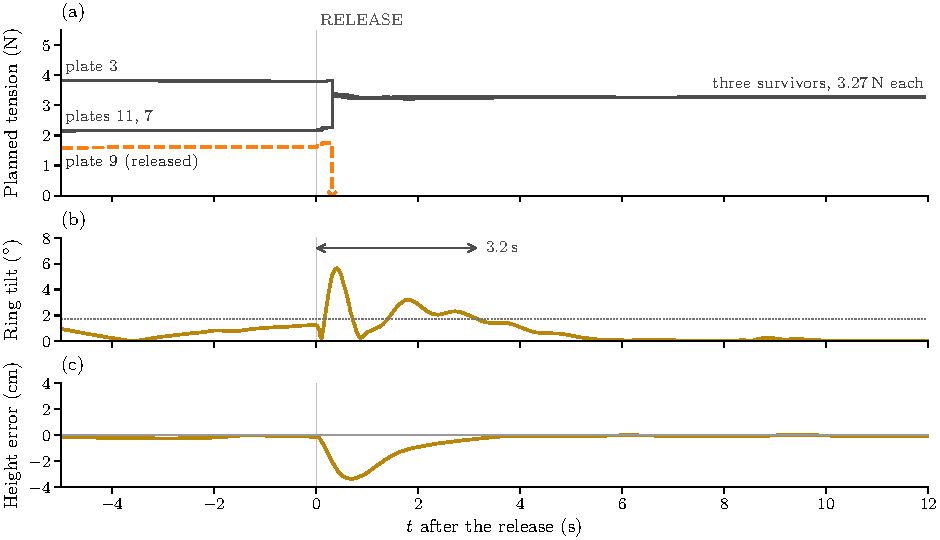
\includegraphics[width=\textwidth]{Images/detach.pdf}
\caption[One release in the twin]{An unannounced release of one UAV of four in the rig twin, hover at 1.0\,m, UAVs on
plates 3, 7, 9 and 11 (Figure~\ref{fig:geometry}), the measured rod pull and the model integral; one run. (a) The
rod tension planned for each UAV; the UAV on plate 9 (dashed) is released at RELEASE and dropped from the plan when the
planner finds the loss, and the three survivors, now an even triangle, share the load equally. (b) Ring tilt; dotted:
the hover's own maximum plus 0.5$^\circ$; arrow: the time until the tilt stays below it. (c) Ring height error
against the 1.0\,m target. The tensions are planned, since the twin does not measure them.}
\label{fig:detach}
\end{figure}


\subsection{The freed UAV's landing}

The freed UAV's own landing, on the rig on 8 October under the old rule and in the twin under the old and the new rule
(Figure~\ref{fig:departed_landing}); the rig's own pair with the new rule waits for the next rig day
(Figure~\ref{fig:rig_departed}).

\begin{figure}[htbp]
\centering
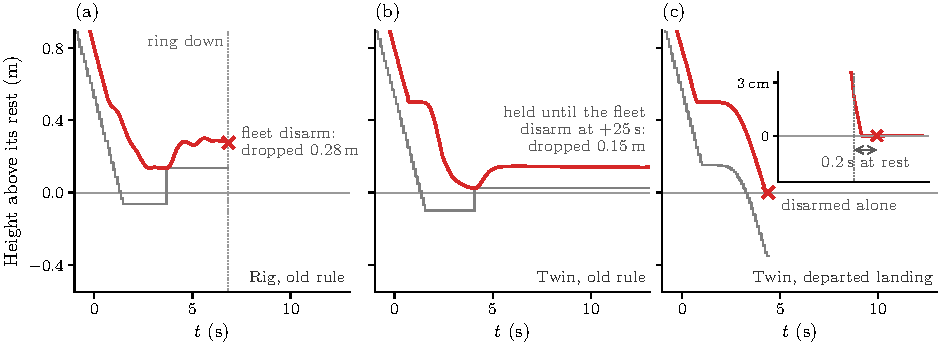
\includegraphics[width=\textwidth]{Images/departed_landing.pdf}
\caption[A freed UAV's own landing, old rule and departed landing]{A UAV landing by itself off the ring, the same UAV
(the fourth) in three cases, aligned where it passes 0.8\,m on the way down; solid: its height above its own resting
height, grey: its height reference until it is disarmed, cross: its disarm, dotted: the ring reaching the floor. (a)
Rig, old rule: its touchdown test fired 0.14\,m above its rest, the reference froze there, the UAV rose to 0.28\,m and
hovered until the fleet's disarm at the end of the landing dropped it 0.28\,m. (b) Twin, old rule: the same stall, held
0.15\,m up for 25\,s until the fleet's disarm dropped it. (c) Twin, departed landing: the reference is pressed below the
resting height until the UAV is there, and it is disarmed alone 0.2\,s after reaching it (inset). The plateau at 0.5\,m
in (b) and (c) is the UAV standing on the tip of its rod before the rod tips over.}
\label{fig:departed_landing}
\end{figure}

\pendingfig{fig:rig_departed}{The freed UAV's own landing on the rig with the departed landing: pushed to its resting
height and disarmed alone.}{the rig's hover and circle releases (L8, L9), the next rig day}

\subsection{The twin against the rig, 8 October}

\begin{figure}[htbp]
\centering
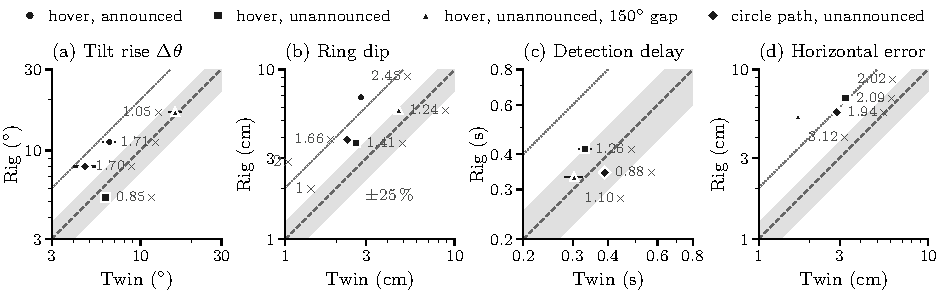
\includegraphics[width=\textwidth]{Images/twin_rig_parity.pdf}
\caption[The twin against the rig]{The rig against its twin for the four releases of 8 October (four UAVs,
0.86\,kg ring at 1.0\,m; one marker per flight; 150$^\circ$ gap: the three left on the ring leave a 150$^\circ$ gap
between two of them), each metric computed the same way from both, on logarithmic axes: $x$, the twin flying the same
configuration (mean of two runs; bar: their range, hidden where it is shorter than the marker); $y$, the rig (one run).
Dashed: $y = x$; grey band: within 25\,\% of the twin; dotted: the rig twice the twin. (a) Tilt rise $\Delta\theta$:
the peak of the ring's tilt-vector departure from its mean over the 5\,s before the release, from the release to the
rig flight's LAND, the twin cut at the same hold. (b) Ring dip: its lowest height error in the 3\,s after the release.
(c) Detection delay: from the release to the planner finding an unannounced release (an announced release needs
none). (d) Horizontal error: the ring's mean distance from its reference over the 10\,s before the release. Within
25\,\% of the twin: the tilt rise of the unannounced hover and 150$^\circ$-gap releases (0.85 and 1.05 times the twin),
the dip of the 150$^\circ$-gap release, and two of the three detection delays (the third is 1.26 times the twin; all
three within 0.1\,s). The announced hover release and the circle release rose 1.7 times the twin; the other three dips
were 1.4--2.5 times the twin's, and the horizontal error was 1.9--3.1 times (5.3--6.8\,cm against 1.7--3.3\,cm).}
\label{fig:twin_rig_parity}
\end{figure}
